\section{Aplicación}\label{Application}
Un autómata de sufijo se puede utilizar para contar el número de \glspl{substring} distintas que se producen en una \gls{string} determinada, también en el reconocimiento de voz, búsqueda de patrones en cantidades masivas de textos en lenguaje natural, la compresión de datos, tareas de extracción de información e identificación musical y emparejamiento en secuencias biológicas (genoma) \cite{wiki:Suffix_automaton}.

\subsection{UVA 719 - Glass Beads}
En competencias de algoritmos, hay muchos problemas relacionados con \glspl{string}, que se resuelven con estructura de datos (\textit{trie}, \textit{suffix tree} y \textit{suffix array}) o programación dinámica. La estructura de datos autómata de sufijo no es tan conocida, pero permite resolver el problema \textit{UVA 719 - Glass Beads}, en el que se debe encontrar la secuencia lexicográfica (orden alfabético) más pequeña entre las cadenas cíclicas. En la Figura \ref{fig:UVA-719-Input-Output} se puede observar el orden lexicográfico de las entradas de ejemplo con su respectiva salida.

\begin{figure}[H]
	\centering
	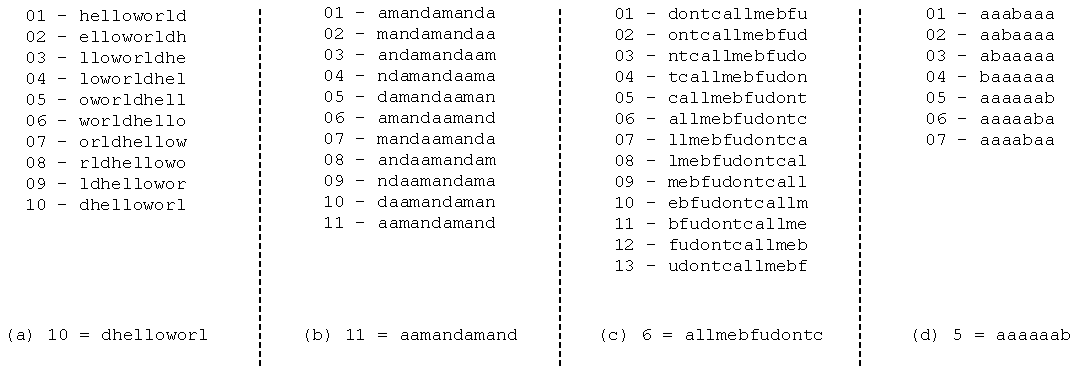
\includegraphics[width=1\linewidth]{doc/Application/img/cases-necklace}
	\caption{Problema: \textit{UVA 719 - Glass Beads}. Casos de entrada que contienen la descripción del collar y el número de la perla que es la primera en la peor separación posible. Cada perla está representada por un carácter en minúscula del alfabeto inglés $(a–z)$, donde $a < b < ... < z$. (a) $helloworld$. (b) $amandamanda$. (c) $dontcallmebfu$. (d) $aaabaaa$. }
	\label{fig:UVA-719-Input-Output}
\end{figure}

La implementación es una traducción a lenguaje \textit{C++ 5.3.0} de los pseudocódigos~\ref{alg:sa} y~\ref{alg:sa_extend}, más la función que retorna el desplazamiento cíclico más pequeño. Se realiza el envío al juez virtual \textit{vjudge}, arrojando un estatus de aceptado en un tiempo de 270ms.

\renewcommand{\lstlistingname}{Implementación}% Listing -> Algorithm
\renewcommand{\lstlistlistingname}{Lista de \lstlistingname s}% List of Listings -> List of Algorithms
\lstset{
	tabsize=2,% tab space width
	basicstyle=\scriptsize,
	showstringspaces=false, % don't mark spaces in strings
	numbers=left, % display line numbers on the left
	numbersep=\intextsep,
	commentstyle=\color{green}, % comment color
	keywordstyle=\color{blue}, % keyword color
	stringstyle=\color{red}, % string color
	xleftmargin=\marginparsep
}
\lstinputlisting[label=SuffixAutomaton, caption=Autómata de sufijo para la solcuión del problema UVA 719 - Glass Beads, language=C++]{doc/Application/code/GlassBeads.cpp}